%\documentclass[handout]{beamer}
\documentclass{beamer}
 
\usetheme[numbering = fraction, progressbar = none, background = light, sectionpage = progressbar]{metropolis}
\usepackage{amsmath}
\usepackage{synttree}
\usepackage{tabu}
\usepackage{graphicx}

\title{Econ 103 -- Statistics for Economists}
\subtitle{Chapter 2 feat. Z Scores and OLS}
\author{Mallick Hossain}
\date{}
\institute{University of Pennsylvania}

\begin{document}

%%%%%%%%%%%%%%%%%%%%%%%%%%%%%%%%%%%%%%%%
\begin{frame}
	\titlepage 
\end{frame} 

%%%%%%%%%%%%%%%%%%%%%%%%%%%%%%%%%%%%%%%%
\begin{frame}
\frametitle{Survey Results}
	To be added soon.
%	\includegraphics[scale=0.5]{survey.jpg}
\end{frame} 

\section{Types of Variables}
%%%%%%%%%%%%%%%%%%%%%%%%%%%%%%%%%%%%%%%%
\begin{frame}
\frametitle{Discussion!}
	\begin{itemize}
		\item What are the differences between the following variables?
		\begin{itemize}
			\item ``Age'' and ``gender''
			\item ``Gender'' and ``class standing''
			\item ``SAT score'' and ``job creation''
		\end{itemize}
	\end{itemize}
\end{frame} 

%%%%%%%%%%%%%%%%%%%%%%%%%%%%%%%%%%%%%%%%
\begin{frame}
\frametitle{A Few Definitions: A Taxonomy of Variables}
	\begin{figure}[htbp]
	\begin{center}
	\scalebox{0.8}{
		\synttree[Variables
			[\begin{tabular}{c}Categorical\\(Qualitative)\end{tabular}
				[Discrete
					[Nominal]
					[Ordinal]
				]%END Discrete
			]%END Categorical
			[\begin{tabular}{c}Numerical\\(Quantitative)\end{tabular}
				[Continuous
					[Ordinal]
					[Interval]
					[Ratio]
				]%END Continuous					
				[Discrete
					[Ordinal]
					[Interval]
					[Ratio]
				]%END Discrete
			]%END numerical
		]%END tree
		}
		\end{center}
	\end{figure}
\end{frame}

%%%%%%%%%%%%%%%%%%%%%%%%%%%%%%%%%%%%%%%%
\begin{frame}
\frametitle{Definitions}
	\begin{itemize}
		\item \textbf{Discrete:} Can be a countable number of values
		\item \textbf{Continuous:} Can take on any value
	\end{itemize}
\end{frame}

%%%%%%%%%%%%%%%%%%%%%%%%%%%%%%%%%%%%%%%%
\begin{frame}
\frametitle{Discussion!}
	Can you order the following from weakest to strongest? 
	\alert{Interval, Nominal, Ordinal, Ratio.}
\end{frame}

%%%%%%%%%%%%%%%%%%%%%%%%%%%%%%%%%%%%%%%%
\begin{frame}
\frametitle{From Weakest to Strongest}
	\begin{itemize}[<+->]
		\item \textbf{Nominal:} no order to the categories
		\item \textbf{Ordinal:} categories with natural order
		\item \textbf{Interval:} only differences meaningful, no natural zero
		\item \textbf{Ratio:} differences and ratios meaningful, natural zero
	\end{itemize}
\end{frame}

\section{Summary Statistics}
%%%%%%%%%%%%%%%%%%%%%%%%%%%%%%%%%%%%%%%
\begin{frame}
\frametitle{Definitions}
	\begin{enumerate}
		\item Measures of Central Tendency
		\begin{itemize}
			\item \textbf{Mean:} the average (``balance point'')
			$$
			\bar{x} = \frac{1}{n} \sum_{i=1}^n x_i
			$$
			\item \textbf{Median:} the middle observation (if data has even number of 							observations, take the mean of the middle two observations)
		\end{itemize}
	\end{enumerate}
\end{frame}

%%%%%%%%%%%%%%%%%%%%%%%%%%%%%%%%%%%%%%%
\begin{frame}
\frametitle{Definitions}
	\begin{enumerate}
	\setcounter{enumi}{1}
		\item Percentiles
		$$
		P^{th} \text{Percentile = Value in}  \left(P/100\right)\cdot (n+1)^{th} \text{Ordered 					Position}
		$$
	\end{enumerate}
\end{frame}

%%%%%%%%%%%%%%%%%%%%%%%%%%%%%%%%%%%%%%%%
\begin{frame}
\frametitle{An Example: n = 12}
	$$
	\begin{array}{cccccccccccc}
		60 & 63 & \alert{65} & \alert{67} & 70 & 72 & 75 & 75 & 80 & 82 & 84 & 85
	\end{array}
	$$
	\begin{eqnarray*}
		\mbox{Q}_1 &=& \mbox{value in the } 0.25(n+1)^{th}\mbox{ ordered position}\\
			&=& \mbox{value in the } 3.25^{th}\mbox{ ordered position}\\
			&=& 0.75 * 65 + 0.25 * 67\\
			&=& 65.5
	\end{eqnarray*}
\end{frame}

%%%%%%%%%%%%%%%%%%%%%%%%%%%%%%%%%%%%%%%
\begin{frame}
\frametitle{Definitions}
	\begin{enumerate}
	\setcounter{enumi}{2}
		\item Measures of Spread
		\begin{itemize}
			\item \textbf{Variance:} the spread from the mean
			$$
			s^2 = \frac{1}{n-1} \sum_{i = 1}^n (x_i - \bar{x})^2
			$$
			\item \textbf{Standard Deviation:} another way to measure the spread
			$$
			s = \sqrt{s^2}
			$$
			\item \textbf{Range:} the distance between the highest and lowest value
			$$
			Range = \left| x_{max} - x_{min} \right|
			$$
			\item \textbf{Interquartile Range (IQR):} the distance between the upper and lower 					quartiles
			$$
			IQR = \left| x_{75\%} - x_{25\%} \right|
			$$
		\end{itemize}
	\end{enumerate}
\end{frame}

 %%%%%%%%%%%%%%%%%%%%%%%%%%%%%%%%%%%%%%%%
 \begin{frame}
 \frametitle{Why Squares?}
	 \begin{center}
	 	\fbox{$\displaystyle s^2 = \frac{1}{n - 1} \sum_{i = 1}^n (x_i - \bar{x})^2$}
	 \end{center}
	\onslide<2-> \begin{alertblock}{What's Wrong With This?}
	 	\begin{align*}
	 		\frac{1}{n - 1} \sum_{i = 1}^n (x_i - \bar{x}) &= \frac{1}{n - 1} \left[\sum_{i = 1}^n x_i - 					\sum_{i = 1}^n \bar{x} \right] = \frac{1}{n - 1} \left[ \sum_{i = 1}^n x_i  - n\bar{x} \right]
	 		\\
	 		&= \frac{1}{n - 1} \left[ \sum_{i = 1}^n x_i  - n \cdot \frac{1}{n} \sum_{i = 1}^n x_i \right]
	 		\\ 
	 		&= \frac{1}{n - 1} \left[ \sum_{i = 1}^n x_i  -  \sum_{i = 1}^n x_i \right] = 0
	 	\end{align*}
	 \end{alertblock}
\end{frame}

%%%%%%%%%%%%%%%%%%%%%%%%%%%%%%%%%%%%%%%
\begin{frame}
\frametitle{Definitions}
	\begin{enumerate}
	\setcounter{enumi}{3}
		\item Measure of Symmetry
		\begin{itemize}
			\item \textbf{Skewness:} a measure of symmetry, positive values means the right tail is 				longer and vice versa
			$$
			Skewness = \frac{1}{n}\frac{\sum_{i = 1}^n (x_i - \bar{x})^3}{s^3}
			$$
		\end{itemize}
	\end{enumerate}
\end{frame}

% %%%%%%%%%%%%%%%%%%%%%%%%%%%%%%%%%%%%%%%%
 \begin{frame}
 \frametitle{Skewness -- A Measure of Symmetry}
	 \begin{center}
	 	\fbox{$\displaystyle\mbox{Skewness} = \frac{1}{n}\frac{\sum_{i = 1}^n (x_i - \bar{x})^3}				{s^3}$}
	 \end{center}
	 \begin{block}{What do the values indicate?}
	 	Zero $\Rightarrow$ symmetry, positive right-skewed, negative left-skewed.
	 \end{block}
	 \begin{block}{Why cubed?}
	 	To get the desired sign.
	 \end{block}
	 \begin{block}{Why divide by $s^3$?}
	 	So that skewness is unitless
	 \end{block}
	 \begin{block}{Rule of Thumb}
	 	Typically (but not always), right-skewed $\Rightarrow$ mean $>$ median
	 	\\ 
	 	left-skewed $\Rightarrow$ mean $<$ median
	 \end{block}
 \end{frame}

%%%%%%%%%%%%%%%%%%%%%%%%%%%%%%%%%%%%%%%
\begin{frame}
\frametitle{Definitions}
	\begin{enumerate}
	\setcounter{enumi}{4}
		\item Relationship between variables (to be covered later)
		\begin{itemize}
			\item \textbf{Covariance:} how two variables vary together
			\item \textbf{Correlation:} normalized version of covariance (can only range between -1 			and +1)
			\item \textbf{Regression:} an estimation of how two variables are related
			\item \alert{We'll cover these in-depth later in the semester}
		\end{itemize}
	\end{enumerate}
\end{frame}

\section{Charts}
%%%%%%%%%%%%%%%%%%%%%%%%%%%%%%%%%%%%%%%
\begin{frame}
\frametitle{Some Data Visualization Quotes}
	\begin{enumerate}
		\item ``Overload, clutter, and confusion are not attributes of information, they are failures 			of design'' --Edward Tufte
		
		\medskip
		
		\item ``...few people will appreciate the music if I just show them the notes. Most of us 				need to listen to the music to understand how beautiful it is. But often, that's how we 				present statistics; we just show the notes we don't play the music.'' --Hans Rosling
	\end{enumerate}
\end{frame}

%%%%%%%%%%%%%%%%%%%%%%%%%%%%%%%%%%%%%%%
\begin{frame}
\frametitle{An Illustration}
	\url{https://i.imgur.com/W4BKCVU.gif}	
\end{frame}

%%%%%%%%%%%%%%%%%%%%%%%%%%%%%%%%%%%%%%%
\begin{frame}
\frametitle{Before and After}
	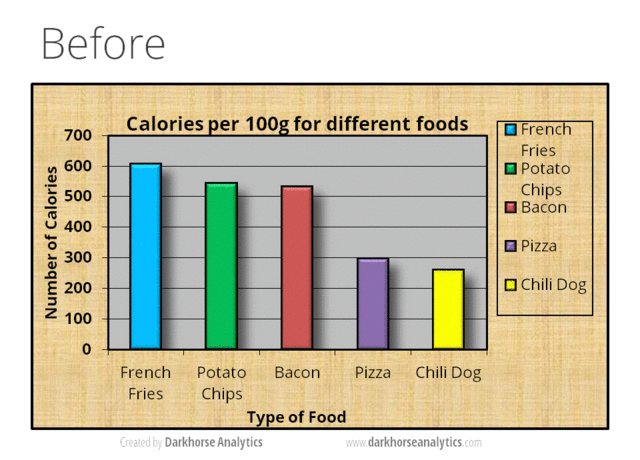
\includegraphics[width = \textwidth]{./images/designBefore.png}
\end{frame}

%%%%%%%%%%%%%%%%%%%%%%%%%%%%%%%%%%%%%%%
\begin{frame}
\frametitle{Before and After}
	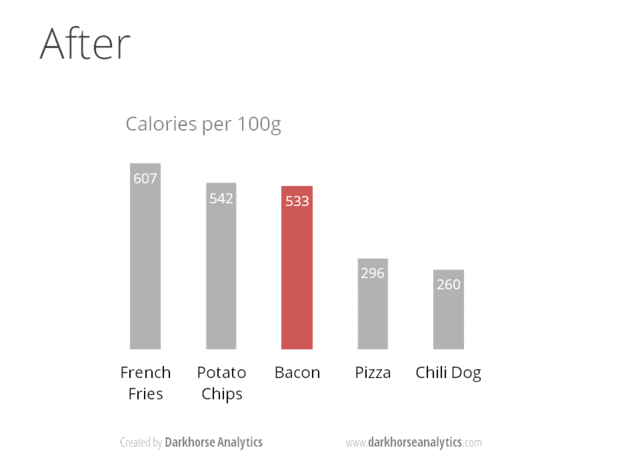
\includegraphics[width = \textwidth]{./images/designAfter.png}
\end{frame}

%%%%%%%%%%%%%%%%%%%%%%%%%%%%%%%%%%%%%%%
\begin{frame}
\frametitle{Illustrating with Charts (Box and Whisker Chart)}
	\begin{figure}
		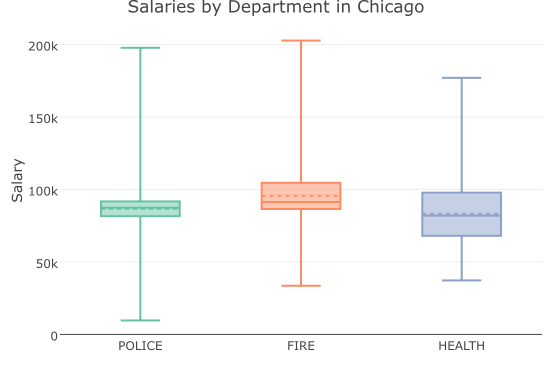
\includegraphics[scale = 0.5]{./images/chicagoBoxPlot.png}
	\end{figure}
\end{frame}

%%%%%%%%%%%%%%%%%%%%%%%%%%%%%%%%%%%%%%%
\begin{frame}
\frametitle{Illustrating with Charts (Histogram)}
	\begin{figure}
		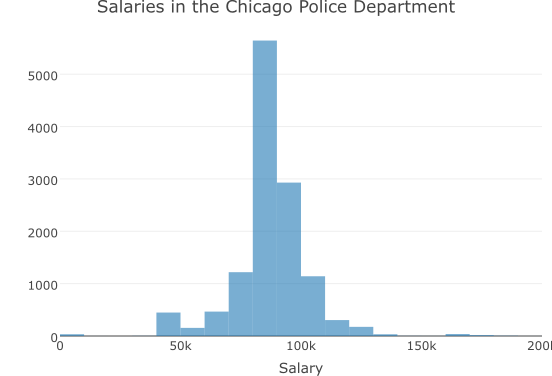
\includegraphics[scale = 0.5]{./images/chicagoHistogram.png}
	\end{figure}
\end{frame}

%%%%%%%%%%%%%%%%%%%%%%%%%%%%%%%%%%%%%%%
\begin{frame}
\frametitle{Histograms are \emph{Really} Important}
	\begin{enumerate}
		\item Histograms show the frequency of different observations
		\item \alert{Important Choice:} How many bins?
	\end{enumerate}
\end{frame}

%%%%%%%%%%%%%%%%%%%%%%%%%%%%%%%%%%%%%%%
\begin{frame}
\frametitle{Too Few Bins (Oversmoothing)}
	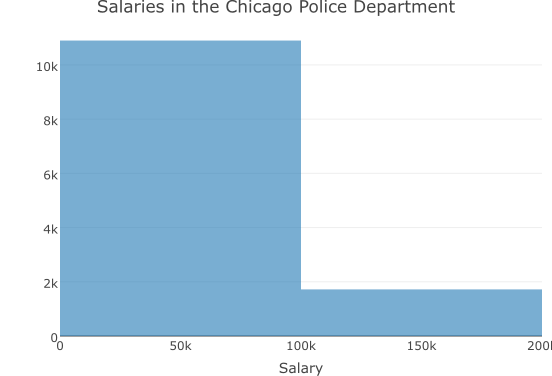
\includegraphics[width = \textwidth]{./images/histogramFew.png}
\end{frame}

%%%%%%%%%%%%%%%%%%%%%%%%%%%%%%%%%%%%%%%
\begin{frame}
\frametitle{Too Many Bins (Undersmoothing)}
	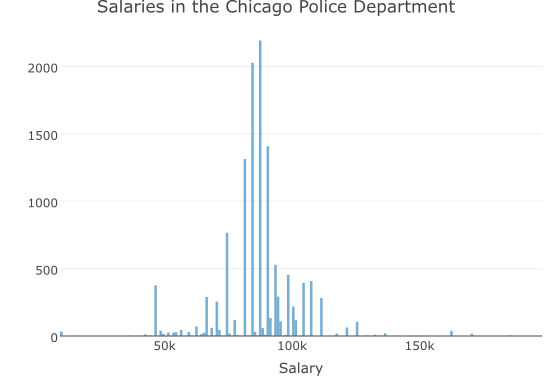
\includegraphics[width = \textwidth]{./images/histogramMany.png}
\end{frame}

%%%%%%%%%%%%%%%%%%%%%%%%%%%%%%%%%%%%%%%
\begin{frame}
\frametitle{Just Right! (Usually around 20 bins or so)}
	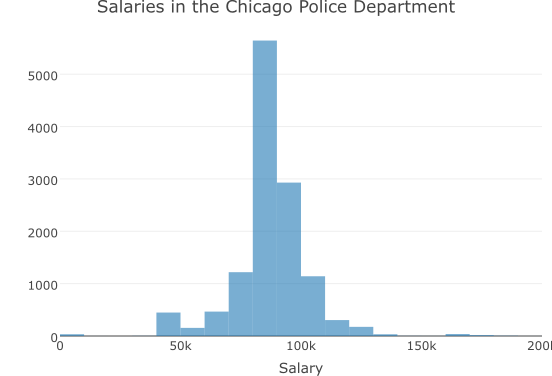
\includegraphics[width = \textwidth]{./images/histogramRight.png}
\end{frame}

%%%%%%%%%%%%%%%%%%%%%%%%%%%%%%%%%%%%%%%
\begin{frame}
\frametitle{Questions to Ask Yourself about Each Summary Statistic}
	\begin{enumerate}
		\item What does it measure?
		\item What are its units compared to those of the data?
		\item How do its units change if those of the data change?
		\item What are the benefits and drawbacks of this statistic?
	\end{enumerate}
	\vspace{2em}
	\alert{Some of the information regarding items 2 and 3 is on the homework rather than in the 		slides because working it out for yourself is a good way to check your understanding.}
\end{frame}

\section{Outliers}
%%%%%%%%%%%%%%%%%%%%%%%%%%%%%%%%%%%%%%%%
\begin{frame}
\frametitle{What is an Outlier?}
	\begin{center}
		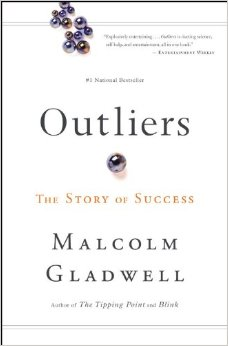
\includegraphics[scale = 0.4]{./images/outliers.jpg}
	\end{center}
	\centering
	\textbf{Outlier:} A very unusual observation relative to the other observations in the dataset 		(i.e.\ very small or very big).
\end{frame}

%%%%%%%%%%%%%%%%%%%%%%%%%%%%%%%%%%%%%%%%
\begin{frame}
\frametitle{Which Summary Stats are Sensitive to Outliers?}
	\begin{itemize}
		\item Assume our data is 1, 2, 3, 4, 5. What are our summary stats (mean, median, variance, 			range, IQR)
		\item What will be affected if the data includes an outlier and becomes 1, 2, 3, 4, 4990?
	\end{itemize}
\end{frame}

%%%%%%%%%%%%%%%%%%%%%%%%%%%%%%%%%%%%%%%%
\begin{frame}
\frametitle{Which Summary Stats are Sensitive to Outliers?}
	\begin{itemize}[<+->]
		\item Mean changes from 3 to 1000
		\item Median remains at 3
		\item Variance changes from 2.5 to 4,975,032
		\item Range changes from 4 to 4889
		\item IQR remains at 2
		\item \alert{When Does the Median Change? IQR?}
		\begin{itemize}
			\item Ranks would have to change.
		\end{itemize}
	\end{itemize}
\end{frame}

%%%%%%%%%%%%%%%%%%%%%%%%%%%%%%%%%%%%%%%%
\begin{frame}
\frametitle{Summary of Sensitivity}
	\begin{block}{Variance}
		Essentially the average squared distance from the mean. Sensitive to both skewness and 			outliers.
	\end{block}
	\begin{block}{Standard Deviation}
		$\sqrt{\mbox{Variance}}$, but more convenient since \alert{same units as data}
	\end{block}
	\begin{block}{Range}
		Difference between larges and smallest observations. \emph{Very} sensitive to outliers. 		
	\end{block}
	\begin{block}{Interquartile Range}
		Range of middle 50\% of the data. Insensitive to outliers, skewness. 
	\end{block}
\end{frame}

\section{Sample vs. Population}
 %%%%%%%%%%%%%%%%%%%%%%%%%%%%%%%%%%%%%%%%
\begin{frame}
\frametitle{Essential Distinction: Sample vs.\ Population}
	For now, you can think of the population as a list of $N$ objects:\\
		\alert{$\mbox{Population: }x_1, x_2, \hdots, x_N$}\\
	from which we draw a sample of size $n<N$ objects:\\
		\alert{$\mbox{Sample: } x_1, x_2, \hdots, x_n$}
	\vspace{3em}
	\begin{alertblock}{Important Point:}
		Later in the course we'll be more formal by considering \alert{probability models} that 				represent the \alert{\emph{act of sampling}} from a population rather than thinking of a 				population as a list of objects. Once we do this we will no longer use the notation $N$ as 			the population will be \alert{\emph{conceptually infinite}}.
	\end{alertblock}
\end{frame}

%%%%%%%%%%%%%%%%%%%%%%%%%%%%%%%%%%%%%%%%
\begin{frame}
\frametitle{Essential Distinction: Parameter vs.\ Statistic}
	$N$ individuals in the Population, $n$ individuals in the Sample:
	\bigskip
	\begin{tabular}{l|l|l}
		&\textbf{Parameter} (Population)&\textbf{Statistic} (Sample)\\
		\hline
		Mean & $\displaystyle \mu = \frac{1}{N} \sum_{i = 1}^N x_i$	& $\displaystyle \bar{x} = 				\frac{1}{n} \sum_{i = 1}^n x_i$ 
		\\
		Var.\ &$ \displaystyle \sigma^2 = \frac{1}{N}\sum_{i = 1}^N (x_i - \mu)^2$ &$ \displaystyle 			s^2 = \frac{1}{n - 1}\sum_{i = 1}^n(x_i - \bar{x})^2$
		\\
		S.D.\ & $ \displaystyle \sigma = \sqrt{\sigma^2}$ &$ \displaystyle s = \sqrt{s^2}$ 
	\end{tabular}
	\bigskip	
	\begin{alertblock}{Key Point}
		We  use a \alert{sample} $x_1, \hdots, x_n$ to calculate \alert{statistics} (e.g.\ $\bar{x}$, 				$s^2$, $s$) that serve as \alert{estimates} of the corresponding population 							\alert{parameters} (e.g.\ $\mu$, $\sigma^2$, $\sigma$).
	\end{alertblock}
\end{frame}

%%%%%%%%%%%%%%%%%%%%%%%%%%%%%%%%%%%%%%%%
\begin{frame}
\frametitle{Why Do Sample Variance and Std.\ Dev.\ Divide by $n - 1$? }
	\begin{align*}
		\sigma^2 &= \frac{1}{N}\sum_{i = 1}^N (x_i - \mu)^2
		\\
		s^2 &= \frac{1}{n - 1}\sum_{i = 1}^n(x_i - \bar{x})^2
	\end{align*}
	\alert{There is an important reason for this, but explaining it requires some concepts we 				haven't learned yet. }
\end{frame}

%%%%%%%%%%%%%%%%%%%%%%%%%%%%%%%%%%%%%%%%
\begin{frame}
\frametitle{Some Intuition}
	\begin{itemize}
		\item \textbf{Intuition 1:} If we only had one data point, what would be the sample 					variance? Would it even be defined?
		\item \textbf{Intuition 2:} We know that the deviations from the sample mean sum to zero 			(see discussion of why variance is squared). Hence, we only need to know $n - 1$ of the 				deviations since the last one will be whatever it takes to make the sum of them equal to 0. 			Hence, it would be proper to divide by $n - 1$ instead of $n$
	\end{itemize}
\end{frame}

\section{Z Scores}
%%%%%%%%%%%%%%%%%%%%%%%%%%%%%%%%%%%%%%%%
\begin{frame}
\frametitle{Why Mean and Variance (and Std.\ Dev.\ )?}
	\begin{alertblock}{Empirical Rule}
	For large populations that are approximately bell-shaped, standard deviation tells where most 		observations will be relative to the mean:
		\begin{itemize}
			\item $\approx$ 68\% of observations are in the interval $\mu \pm \sigma$
			\item $\approx$ 95\% of observations are in the interval $\mu \pm 2\sigma$
			\item Almost all of observations are in the interval $\mu \pm 3\sigma$
		\end{itemize}
	\end{alertblock}
\end{frame}

%%%%%%%%%%%%%%%%%%%%%%%%%%%%%%%%%%%%%%%%
\begin{frame}
\frametitle{Standard Deviations}
	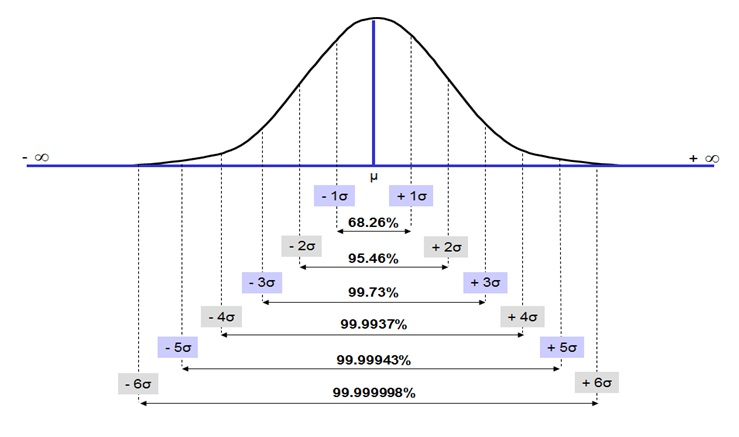
\includegraphics[width = \textwidth]{./images/six_sigma_normal_distribution.jpg}
\end{frame}

%%%%%%%%%%%%%%%%%%%%%%%%%%%%%%%%%%%%%%%%
\begin{frame}
\frametitle{Z-scores: How many standard deviations from the mean?}
	$$
	z _i= \frac{x_i - \bar{x}}{s}
	$$
	\pause
	\begin{block}{Unitless}
		Allows comparison of variables with different units.
	\end{block}
	\pause
	\begin{block}{Detecting Outliers}
		Measures how ``extreme'' one observation is relative to the others.
	\end{block}
	\pause
	\begin{block}{Linear Transformation}
	\end{block}
\end{frame}

%%%%%%%%%%%%%%%%%%%%%%%%%%%%%%%%%%%%%%%%
\begin{frame}
\frametitle{What is the sample mean of the z-scores?}
	\begin{align*}
	 \only<2->{\bar{z} &= \frac{1}{n} \sum_{i = 1}^n z_i = \frac{1}{n} \sum_{i = 1}^n \frac{x_i - \bar{x}}		{s}= \frac{1}{n\cdot s} \left[\sum_{i = 1}^n x_i  - \sum_{i = 1}^n \bar{x}  \right]
	 \\}
	\only<3->{&= \frac{1}{n\cdot s} \left[\sum_{i = 1}^n x_i  - n\bar{x}  \right] = \frac{1}{n\cdot s} 			\left[\sum_{i = 1}^n x_i - n\cdot \frac{1}{n} \sum_{i = 1}^n x_i  \right] 
	 \\}
 	\only<4->{&= \frac{1}{n\cdot s} \left[\sum_{i = 1}^n x_i -  \sum_{i = 1}^n x_i  \right]  = 0}
	\end{align*}
\end{frame}

%%%%%%%%%%%%%%%%%%%%%%%%%%%%%%%%%%%%%%%%
\begin{frame}
\frametitle{What is the variance of the z-scores?}
	\begin{align*}
		\only<2->{s^2_z &= \frac{1}{n - 1}\sum_{i = 1}^n (z_i - \bar{z})^2 = \frac{1}{n - 1}\sum_{i = 				1}^n z_i^2 = 	\frac{1}{n - 1} \sum_{i = 1}^n \left(\frac{x_i - \bar{x}}{s_x}\right)^2
		\\}
		\only<3->{&= \frac{1}{s_x^2} \left[ \frac{1}{n - 1} \sum_{i = 1}^n \left(x_i - \bar{x}\right)^2 				\right] = \frac{s_x^2}{s_x^2} = 1}
		\end{align*}
	\vspace{5em}
	\only<4->{\alert{So what is the \emph{standard deviation} of the z-scores? \hfill  }}
\end{frame}

%%%%%%%%%%%%%%%%%%%%%%%%%%%%%%%%%%%%%%%%
\begin{frame}
\frametitle{Population Z-scores and the Empirical Rule: $\mu \pm 2\sigma$}
	If we knew the population mean $\mu$ and standard deviation $\sigma$ we could create a 			\alert{\emph{population version}} of a z-score. This leads to an important way of rewriting the 		Empirical Rule:
	\vspace{2em}
	\alert{Bell-shaped population $\Rightarrow$ approx.\ 95\% of observations $x_i$ satisfy}
	\begin{align*}
	\mu - 2\sigma &\leq x_i \leq \mu + 2\sigma
	\\
	\\
	-2 \sigma &\leq x_i -\mu \leq 2\sigma
	\\
	\\
	-2 &\leq \frac{x_i - \mu}{\sigma} \leq 2
	\end{align*}
\end{frame}

\section{Covariance and Correlation}
%%%%%%%%%%%%%%%%%%%%%%%%%%%%%%%%%%%%%%%%
\begin{frame}
\frametitle{Covariance and Correlation: Linear Dependence Measures}
	\begin{block}{Two Samples of Numeric Data}
		$x_1, \hdots, x_n$ and $y_1, \hdots, y_n$
	\end{block}
	\begin{block}{Dependence}
		Do $x$ and $y$ both tend to be large (or small) at the same time?
	\end{block}
	\begin{block}{Key Point}
		Use the idea of centering and standardizing to decide what ``big'' or ``small'' means in this 			context.
	\end{block}
\end{frame}

%%%%%%%%%%%%%%%%%%%%%%%%%%%%%%%%%%%%%%%%
\begin{frame}
\frametitle{Are Engine Cylinders and Horsepower Related?}
	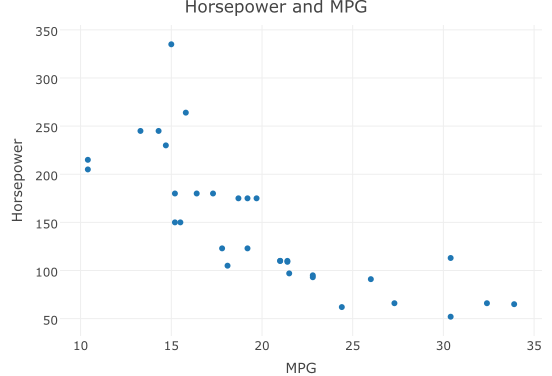
\includegraphics[scale=0.5]{./images/cars.png}
\end{frame}

%%%%%%%%%%%%%%%%%%%%%%%%%%%%%%%%%%%%%%%%
\begin{frame}
\frametitle{Recall Formulas}
	\begin{align*}
		\bar{x} &= \frac{1}{n} \sum_{i = 1}^n x_i
		\\
		\bar{y} &= \frac{1}{n} \sum_{i = 1}^n y_i
		\\
		s_x &= \sqrt{\frac{1}{n - 1} \sum_{i = 1}^n (x_i - \bar{x})^2}
		\\
		s_y &= \sqrt{\frac{1}{n - 1} \sum_{i = 1}^n (y_i - \bar{y})^2}
	\end{align*}
\end{frame}

%%%%%%%%%%%%%%%%%%%%%%%%%%%%%%%%%%%%%%%%
\begin{frame}
\frametitle{Covariance}
	$$
	s_{xy} = \frac{1}{n-1} \sum_{i=1}^n (x_i -\bar{x})(y_i - \bar{y})
	$$
	\begin{itemize}
		\item Centers each observation around its mean and multiplies.
		\item Zero $\Rightarrow$ no linear dependence
		\item Positive $\Rightarrow$ positive linear dependence
		\item Negative $\Rightarrow$ negative linear dependence
		\item Population parameter: $\sigma_{xy}$
		\item Units?
	\end{itemize}
\end{frame}

%%%%%%%%%%%%%%%%%%%%%%%%%%%%%%%%%%%%%%%%
\begin{frame}
\frametitle{Correlation}
	$$
	r_{xy} = \frac{1}{n - 1} \sum_{i = 1}^n \left(\frac{x_i  - \bar{x}}{s_x}\right)\left(\frac{y_i - \bar{y}}			{s_y}\right) = \frac{s_{xy}}{s_x s_y}
	$$
	\begin{itemize}
		\item Centers \emph{and} standardizes each observation 
		\item Bounded between -1 and 1
		\item Zero $\Rightarrow$ no linear dependence
		\item Positive $\Rightarrow$ positive linear dependence
		\item Negative $\Rightarrow$ negative linear dependence
		\item Population parameter: $\rho_{xy}$
		\item Unitless
	\end{itemize}
\end{frame}

%%%%%%%%%%%%%%%%%%%%%%%%%%%%%%%%%%%%%%%%
\begin{frame}
\frametitle{Game!}
	\url{guessthecorrelation.com}
\end{frame}

\section{Introduction to Regression}
%%%%%%%%%%%%%%%%%%%%%%%%%%%%%%%%%%%%%%%%
\begin{frame}
\frametitle{Least Squares Regression -- Predict Using a Line}
	\begin{center}
		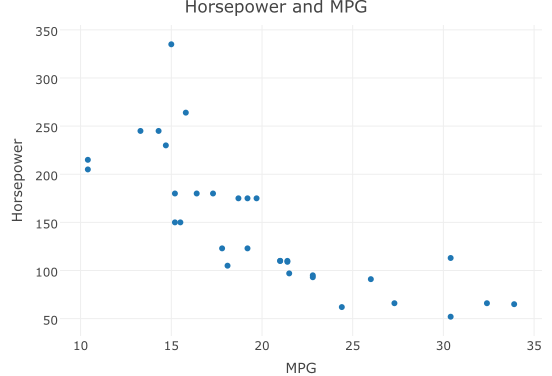
\includegraphics[scale=0.4]{./images/cars.png}
	\end{center}
	\begin{itemize}
		\item In order to fit a line through this, we need to estimate $y = a + bx$
		\item How do we find $a$ and $b$?
	\end{itemize}
\end{frame}
	
%%%%%%%%%%%%%%%%%%%%%%%%%%%%%%%%%%%%%%%%
\begin{frame}
\frametitle{Finding $a$ and $b$}
	\begin{itemize}
		\item Linear regression chooses the slope ($b$) and intercept ($a$) that \alert{minimize the 		sum of squared vertical deviations}
		$\displaystyle\sum_{i = 1}^n d_i^2 = \sum_{i = 1}^n (y_i - a - b x_i)^2$
		\medskip
		\item Why do we square the deviations?
	\end{itemize}
\end{frame}

%%%%%%%%%%%%%%%%%%%%%%%%%%%%%%%%%%%%%%%%
\begin{frame}
\frametitle{Important Point About Notation}
  	$$
  	\boxed{\underset{a, b}{\mbox{minimize }}\sum_{i = 1}^n d_i^2 = \sum_{i = 1}^n 
  	(y_i - a - b x_i)^2}
  	$$
	$$
	\boxed{\hat{y} = a + bx}
	$$
	\begin{itemize}
		\item $(x_i, y_i)_{i = 1}^n$ are the \alert{observed data}
		\item $\widehat{y}$ is our \alert{prediction} for a given value of $x$
		\item Neither $x$ nor $\widehat{y}$ needs to be in out dataset!
	\end{itemize}
\end{frame}

%%%%%%%%%%%%%%%%%%%%%%%%%%%%%%%%%%%%%%%%
\begin{frame}
\frametitle{Prediction 28 MPG?}
	\begin{figure}
		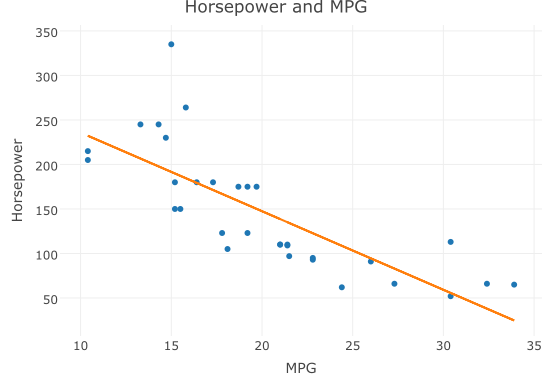
\includegraphics[scale = 0.4]{./images/carsFitted.png}
	\end{figure}
	$$
	\widehat{hp} = 324.08 - 8.83 mpg
	$$
	\only<2->{\alert{
	$$
	76.84 = 324.08 - 8.83 * 28
	$$
	}}
\end{frame}

%%%%%%%%%%%%%%%%%%%%%%%%%%%%%%%%%%%%%%%%
\begin{frame}
\frametitle{You Need to Know How To Derive This}
	\alert{Minimize the sum of squared vertical deviations from the line:}
	$$
	\min_{a,b}  \sum_{i=1}^n (y_i - a - b x_i)^2
	$$
	How should we proceed? Select all that apply.
	\begin{enumerate}[(a)]
		\item Differentiate with respect to $x$
		\item Differentiate with respect to $y$
		\item Differentiate with respect to $a$
		\item Differentiate with respect to $b$
		\item You can't fool me! You can't solve this with calculus.
	\end{enumerate}
\end{frame}

%%%%%%%%%%%%%%%%%%%%%%%%%%%%%%%%%%%%%%%%
\begin{frame}
\begin{block}{Objective Function}
$$\displaystyle \min_{a,b}  \sum_{i=1}^n (y_i - a - b x_i)^2$$
\end{block}
\begin{block}{FOC with respect to $a$}\pause
\begin{eqnarray*}
	-2 \sum_{i=1}^n\left(y_i - a -bx_i\right) &=& 0 \\\pause
	\sum_{i=1}^n y_i - \sum_{i=1}^n a - b\sum_{i=1}^n x_i &=& 0 \\\pause
	\frac{1}{n} \sum_{i=1}^n y_i - \frac{na}{n} -  \frac{b}{n} \sum_{i=1}^n x_i &=& 0\\\pause
	\bar{y} - a - b\bar{x} &=& 0
\end{eqnarray*}
\end{block}
\end{frame}
%%%%%%%%%%%%%%%%%%%%%%%%%%%%%%%%%%%%%%%%
\begin{frame}

\frametitle{Regression Line Goes Through the Means!}
 \Huge
\begin{equation*}\boxed{\bar{y} = a + b\bar{x}}\end{equation*}
\normalsize
\end{frame}
%%%%%%%%%%%%%%%%%%%%%%%%%%%%%%%%%%%%%%%%
\begin{frame}
  \frametitle{Substitute $a = \bar{y} - b \bar{x}$}
  \small
\begin{eqnarray*}
	\sum_{i=1}^n (y_i - a - b x_i)^2 &=& \pause\sum_{i=1}^n (y_i - \bar{y} + b\bar{x} - b x_i)^2\\
	&=&\pause\sum_{i=1}^n \left[ \left(y_i - \bar{y}\right) - b\left(x_i - \bar{x}\right) \right]^2
\end{eqnarray*}
\alert{FOC wrt $b$}
\begin{eqnarray*}\pause
	-2\sum_{i=1}^n \left[\left(y_i - \bar{y}\right) - b\left(x_i - \bar{x}\right) \right]\left(x_i - \bar{x} \right) &=& 0\\\pause
	\sum_{i=1}^n \left(y_i - \bar{y}\right)\left(x_i - \bar{x} \right) - b\sum_{i=1}^n \left(x_i - \bar{x}\right)^2 &=& 0\\ \\\pause
	b = \frac{\sum_{i=1}^n \left(y_i - \bar{y}\right)\left(x_i - \bar{x} \right)}{\sum_{i=1}^n \left(x_i - \bar{x}\right)^2}
\end{eqnarray*}
\end{frame}
%%%%%%%%%%%%%%%%%%%%%%%%%%%%%%%%%%%%%%%%
\begin{frame}
\frametitle{Simple Linear Regression}
	\begin{block}{Problem}
	$$\min_{a,b}  \sum_{i=1}^n (y_i - a - b x_i)^2$$
\end{block}
\begin{block}{Solution}
	\begin{eqnarray*}
		b &=& \frac{\sum_{i=1}^n \left(y_i - \bar{y}\right)\left(x_i - \bar{x} \right)}{\sum_{i=1}^n \left(x_i - \bar{x}\right)^2}\\ \\
		a &=& \bar{y} - b\bar{x}
	\end{eqnarray*}
\end{block}
\end{frame}

%%%%%%%%%%%%%%%%%%%%%%%%%%%%%%%%%%%%%%%%
\begin{frame}
	\frametitle{Relating Regression to Covariance and Correlation}
		$$b = \frac{\sum_{i=1}^n \left(y_i - \bar{y}\right)\left(x_i - \bar{x} \right)}{\sum_{i=1}^n \left(x_i - \bar{x}\right)^2} = \frac{\frac{1}{n-1}\sum_{i=1}^n \left(y_i - \bar{y}\right)\left(x_i - \bar{x} \right)}{\frac{1}{n-1}\sum_{i=1}^n \left(x_i - \bar{x}\right)^2} = \frac{s_{xy}}{s_x^2}$$
		
		$$r = \frac{s_{xy}}{s_x s_y} = b \frac{s_x}{s_y}$$
		
\end{frame}
%%%%%%%%%%%%%%%%%%%%%%%%%%%%%%%%%%%%%%%%
\begin{frame}
\frametitle{Comparing Regression, Correlation and Covariance}

\begin{block}{Units}
Correlation is unitless, covariance and regression coefficients ($a, b$) are not. (What are the units of these?)
\end{block}


\begin{block}{Symmetry}
Correlation and covariance are symmetric, regression isn't. (Switching $x$ and $y$ axes changes the slope and intercept.)
\end{block}

\begin{block}{On the Homework}
Regression with z-scores rather than raw data gives $a=0, b = r_{xy}$
\end{block}

\end{frame}
%%%%%%%%%%%%%%%%%%%%%%%%%%%%%%%%%%%%%%%%

\begin{frame}

$\begin{array}{ccccc} s_{xy} = 6,&s_x = 5,& s_y = 2,& \bar{x} = 68,& \bar{y} = 21\end{array}$
\begin{columns}[c]
\column{2.5in}
What is the sample correlation between height ($x$) and handspan ($y$)?
\column{1.8in}
\includegraphics[scale = 0.4]{./images/height_handspan1}
\end{columns}
\alert{$$\phantom{r = \frac{s_{xy}}{s_x s_y} = \frac{6}{4.5\times 2.2} \approx 0.6}$$}
\end{frame}
%%%%%%%%%%%%%%%%%%%%%%%%%%%%%%%%%%%%%%%%
\begin{frame}
$\begin{array}{ccccc} s_{xy} = 6,&s_x = 5,& s_y = 2,& \bar{x} = 68,& \bar{y} = 21\end{array}$
\begin{columns}[c]
\column{2.5in}
What is the sample correlation between height ($x$) and handspan ($y$)?
\column{1.8in}
\includegraphics[scale = 0.4]{./images/height_handspan_zline}
\end{columns}
\alert{$$r = \frac{s_{xy}}{s_x s_y} = \frac{6}{5\times 2} = 0.6$$}
\end{frame}
%%%%%%%%%%%%%%%%%%%%%%%%%%%%%%%%%%%%%%%%
\begin{frame}
$\begin{array}{ccccc} s_{xy} = 6,&s_x = 5,& s_y = 2,& \bar{x} = 68,& \bar{y} = 21\end{array}$
\begin{columns}[c]
\column{2.5in}
What is the value of $b$ for the regression: $$\hat{y}=a+bx$$
where $x$ is height and $y$ is handspan?
\column{1.8in}
\includegraphics[scale = 0.4]{./images/height_handspan1}
\end{columns}
\alert{$$\phantom{b = \frac{s_{xy}}{s_x^2} = \frac{6}{(4.5)^2} = 6/20.25 \approx 0.3}$$}
\end{frame}
%%%%%%%%%%%%%%%%%%%%%%%%%%%%%%%%%%%%%%%%
\begin{frame}
$\begin{array}{ccccc} s_{xy} = 6,&s_x = 5,& s_y = 2,& \bar{x} = 68,& \bar{y} = 21\end{array}$
\begin{columns}[c]
\column{2.5in}
What is the value of $b$ for the regression: $$\hat{y}=a+bx$$
where $x$ is height and $y$ is handspan?
\column{1.8in}
\includegraphics[scale = 0.4]{./images/height_handspan2}
\end{columns}
\alert{$$b = \frac{s_{xy}}{s_x^2} = \frac{6}{5^2} = 6/25 = 0.24 $$}
\end{frame}
%%%%%%%%%%%%%%%%%%%%%%%%%%%%%%%%%%%%%%%%
\begin{frame}
$\begin{array}{ccccc} s_{xy} = 6,&s_x = 5,& s_y = 2,& \bar{x} = 68,& \bar{y} = 21\end{array}$
\begin{columns}[c]
\column{2.5in}
What is the value of $a$ for the regression: $$\hat{y}=a+bx$$
where $x$ is height and $y$ is handspan? (prev.\ slide $b = 0.24$)
\column{1.8in}
\includegraphics[scale = 0.4]{./images/height_handspan1}
\end{columns}
\alert{$$\phantom{a = \bar{y} - b \bar{x} = 20.6 - 0.297 \times 67.6 \approx 0.5}$$}
\end{frame}
%%%%%%%%%%%%%%%%%%%%%%%%%%%%%%%%%%%%%%%%
\begin{frame}
$\begin{array}{ccccc} s_{xy} = 6,&s_x = 5,& s_y = 2,& \bar{x} = 68,& \bar{y} = 21\end{array}$
\begin{columns}[c]
\column{2.5in}
What is the value of $a$ for the regression: $$\hat{y}=a+bx$$
where $x$ is height and $y$ is handspan? (prev.\ slide $b = 0.24$)
\column{1.8in}
\includegraphics[scale = 0.4]{./images/height_handspan2}
\end{columns}
\alert{$$a = \bar{y} - b \bar{x} = 21 - 0.24 \times 68 = 4.68 $$}
\end{frame}
%%%%%%%%%%%%%%%%%%%%%%%%%%%%%%%%%%%%%%%%
\begin{frame}
\alert{$\begin{array}{ccccc} s_{xy} = 6,&s_y = 5,& s_x = 2,& \bar{y} = 68,& \bar{x} = 21\end{array}$}
\begin{columns}[c]
\column{2.5in}
What is the value of $b$ for the regression: $$\hat{y}=a+bx$$
where \alert{$x$ is handspan and $y$ is height? }
\column{1.8in}
\includegraphics[scale = 0.4]{./images/handspan_height}
\end{columns}
\alert{$$\phantom{b = \frac{s_{xy}}{s_x^2} = 6 /2.2^2 \approx 1.2}$$}
\end{frame}
%%%%%%%%%%%%%%%%%%%%%%%%%%%%%%%%%%%%%%%%
\begin{frame}
\alert{$\begin{array}{ccccc} s_{xy} = 6,&s_y = 5,& s_x = 2,& \bar{y} = 68,& \bar{x} = 21\end{array}$}
\begin{columns}[c]
\column{2.5in}
What is the value of $b$ for the regression: $$\hat{y}=a+bx$$
where \alert{$x$ is handspan and $y$ is height? }
\column{1.8in}
\includegraphics[scale = 0.4]{./images/handspan_height2}
\end{columns}
\alert{$$b = \frac{s_{xy}}{s_x^2} = 6 /2^2 = 1.5 $$}
\end{frame}
%%%%%%%%%%%%%%%%%%%%%%%%%%%%%%%%%%%%%%%%
\begin{frame}

\begin{alertblock}{EXTREMELY IMPORTANT}
	\begin{itemize}
		\item Regression, Covariance and Correlation: linear association.
		\item Linear association $\neq$ causation. 
		\item Linear is not the only kind of association!
	\end{itemize}
\end{alertblock}

\centering{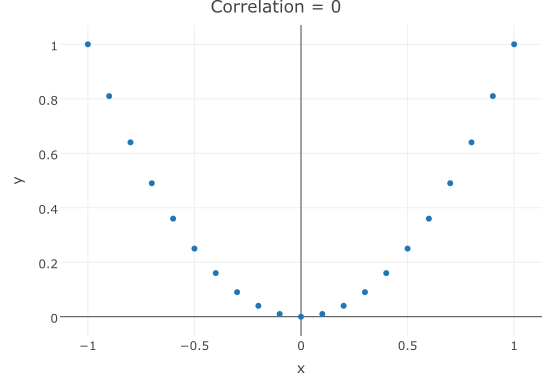
\includegraphics[scale = 0.45]{./images/zero_corr}}

\end{frame}

%%%%%%%%%%%%%%%%%%%%%%%%%%%%%%%%%%%%%%%%
\begin{frame}
  \frametitle{Regression to the Mean and the Regression Fallacy}

  \alert{Please read Chapter 17 of ``Thinking Fast and Slow'' by Daniel Kahnemann which I have posted on Piazza. This reading is fair game on an exam or quiz.}
\end{frame}
%%%%%%%%%%%%%%%%%%%%%%%%%%%%%%%%%%%%%%%%
\begin{frame}

\centering{\includegraphics[scale = 0.46]{./images/pearson}}


\end{frame}

%%%%%%%%%%%%%%%%%%%%%%%%%%%%%%%%%%%%%%%%
%\begin{frame}
%\frametitle{\includegraphics[scale = 0.05]{./images/clicker}}
%
%Suppose a father is very short compared to other fathers (very negative z-score). Would you expect his son to be:
%	\begin{enumerate}[(a)]
%\item Shorter
%\item About as short
%\item Taller
%\end{enumerate}
%\end{frame}

%%%%%%%%%%%%%%%%%%%%%%%%%%%%%%%%%%%%%%%%
%\begin{frame}
%
%\centering{\includegraphics[scale = 0.65]{./images/short_father}}
%
%
%\end{frame}
%
%%%%%%%%%%%%%%%%%%%%%%%%%%%%%%%%%%%%%%%%%
%
%
%\begin{frame}
%
%\centering{\includegraphics[scale = 0.65]{./images/tall_father}}
%
%
%\end{frame}
%
%%%%%%%%%%%%%%%%%%%%%%%%%%%%%%%%%%%%%%%%%
%
%
%\begin{frame}
%
%\centering{\includegraphics[scale = 0.46]{./images/pearson}}
%
%
%\end{frame}
%
%%%%%%%%%%%%%%%%%%%%%%%%%%%%%%%%%%%%%%%%

\begin{frame}
\frametitle{Regression to the Mean}

\begin{block}{Skill and Luck / Genes and Random Environmental Factors}\end{block}


\begin{block}{Unless $r_{xy}=1$, There Is Regression to the Mean}
$$\frac{\hat{y} - \bar{y}}{{s_y}} = r_{xy} \frac{x - \bar{x}}{s_x}$$
\end{block}

\begin{alertblock}{Least-squares Prediction $\hat{y}$ closer to $\bar{y}$ than $x$ is to $\bar{x}$}
\end{alertblock}
You will derive the above formula in this week's homework.
\end{frame}
%%%%%%%%%%%%%%%%%%%%%%%%%%%%%%%%%%%%%%%%
%\begin{frame}
%\frametitle{Regression Fallacy}
%\framesubtitle{For More, See the Document Posted on Piazza}
%\begin{block}{Pre-test}
%Which students are strongest, which are weakest?
%\end{block}
%
%\begin{block}{Intervention} Put the best performing in an enrichment program and the worst performing in a remedial class
%\end{block}
%
%\begin{block}{Post-test}
%The weak students did better than on their first test, but the strong students did \emph{worse}.
%\end{block}
%
%\begin{block}{Mistaken Conclusion}
%Remedial classes are beneficial, enrichment programs are harmful
%\end{block}
%\end{frame}
%%%%%%%%%%%%%%%%%%%%%%%%%%%%%%%%%%%%%%%%
\begin{frame}
  \frametitle{Next Up: Basic Probability}
  Please do the following before our next class:
      \vspace{1em}
  \begin{enumerate}
    \item Complete the ``Odd Questions'' quiz posted on Piazza \texttt{OddQuestions.pdf} -- we'll be discussing these in class.
      \vspace{1em}
    \item If you're rusty on permutations, combinations, etc. from High School math, read this review \footnotesize \url{http://ditraglia.com/Econ103Public/ClassicalProbability.pdf}
  \end{enumerate}
\end{frame}
%%%%%%%%%%%%%%%%%%%%%%%%%%%%%%%%%%%%%%%%


\section{Review}
%%%%%%%%%%%%%%%%%%%%%%%%%%%%%%%%%%%%%%%%
\begin{frame}
\frametitle{Essential Distinction: Parameter vs.\ Statistic}
	$N$ individuals in the Population, $n$ individuals in the Sample:
	\vspace{1em}
	\small
	\begin{tabular}{l|l|l}
		&\textbf{Parameter} (Population)&\textbf{Statistic} (Sample)\\
		\hline
		Mean&$\displaystyle\mu_x = \frac{1}{N} \sum_{i = 1}^N x_i$& $\displaystyle\bar{x} = \frac{1}			{n} \sum_{i = 1}^n x_i$ \\
		Var.\ &$\displaystyle \sigma_x^2 = \frac{1}{N}\sum_{i = 1}^N (x_i - \mu)^2$ &$\displaystyle 			s_x^2 = \frac{1}{n - 1}\sum_{i = 1}^n(x_i - \bar{x})^2$\\
		S.D.\ &$\sigma_x = \sqrt{\sigma_x^2}$ &$s_x = \sqrt{s^2}$ \\
		&&\\
		\hline
		&&\\
		\alert{Cov.\ }&\alert{$\displaystyle \sigma_{xy} = \frac{\sum_{i = 1}^N(x_i - \mu_x)(y_i - 				\mu_y)}{N}$} &\alert{$\displaystyle s_{xy} = \frac{\sum_{i = 1}^n(x_i - \bar{x})(y_i - \bar{y})}			{n - 1}$}\\
		\alert{Corr.\ } & \alert{$\displaystyle \rho = \frac{\sigma_{xy}}{\sigma_x \sigma_y}$}& 					\alert{$\displaystyle r = \frac{s_{xy}}{s_x s_y}$}
	\end{tabular}
\end{frame}

%%%%%%%%%%%%%%%%%%%%%%%%%%%%%%%%%%%%%%%%
\begin{frame}
\frametitle{Related Reading}
	\begin{itemize}
		\item Wonnacott: Chapter 2, Section 4-5 A+B, Section 5-3, Appendix 2-2, and Appendix 2-5
		\item How to Lie with Statistics: Chapters 2, 5, and 6
	\end{itemize}
\end{frame}

%%%%%%%%%%%%%%%%%%%%%%%%%%%%%%%%%%%%%%%%
\end{document}